\appendix

\section{Analysis of the Dataset with Air Speed Measurements at Three Heights}\label{sec:analysis-of-the-dataset-with-air-speed-measurements-at-three-heights}

In this section, we show the results of the analysis of the dataset with air speed measurements at three heights.
Only \num{3063} entries in the \ac{db2} had air speed measurements at three heights with \ac{vr}~$\geq$~\qty{0.2}{\m\per\s}.
A summary of the papers that collected these data is provided in Table~\ref{tab:three_heights_papers}.
The table also shows the number of measurements for each paper and how much (percentage) each study contributed to the dataset.
\begin{table}[htb!]
    \centering
    \begin{tabular}{lrr}
\toprule
Publication & Count & \% Total \\
\midrule
Cena, K., and de Dear, R. J. (1999) & 827 & 27 \\
de Dear, R.J. and Fountain, M.E. (1994) & 704 & 23 \\
Zhang, Y., Chen, H., Meng, Q. (2013) & 465 & 15 \\
Zhang, Y. et al. (2010) & 416 & 14 \\
Schiller (Brager), G. (1990) & 304 & 10 \\
Donnini, G. et al. (1996) & 192 & 6 \\
Tartarini, F., Cooper, P., Fleming, R. (2018) & 113 & 4 \\
Benton, C. C. and Brager, G. S. (1994) & 30 & 1 \\
\bottomrule
\end{tabular}

    \caption{The number of entries used in this analysis grouped by publication.
    We did not include papers with less than \num{5} entries.}
    \label{tab:three_heights_papers}
\end{table}
The paper by Cena et al.\ (1999), de Dear et al.\ (1994), and Zhang et al.\ (2013 and 2010) contributed the most to the dataset (\qty{79}{\percent}).
The air speed distribution at the three heights for each paper is shown in Figure~\ref{fig:boxenplot_wind_speed_three_heights}.
\begin{figure}[htb!]
    \centering
    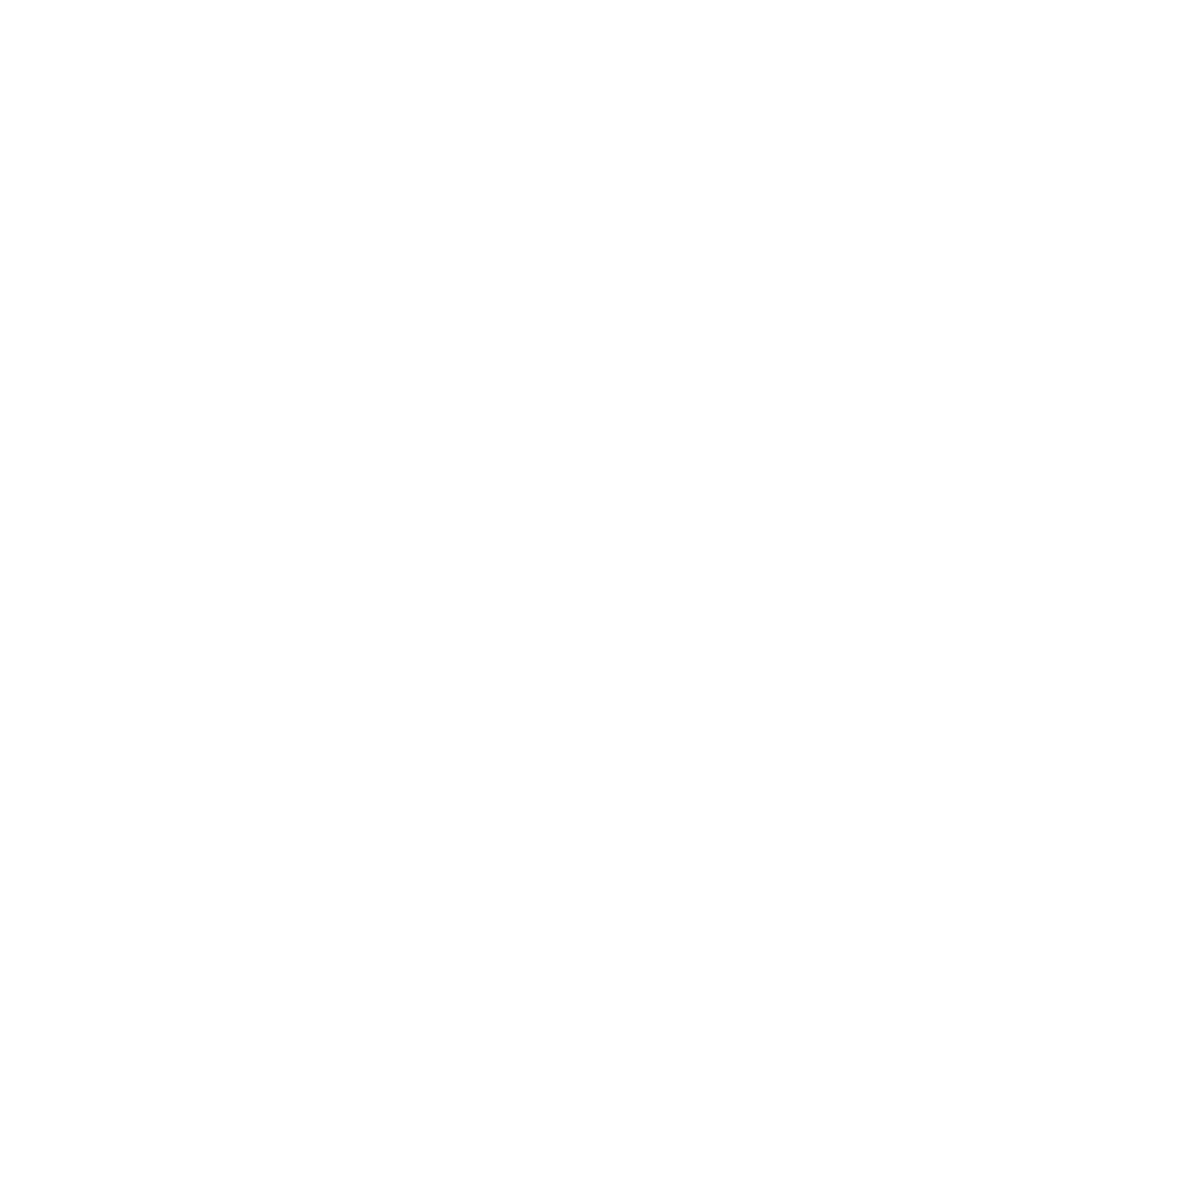
\includegraphics[width=\textwidth]{figures/boxenplot_wind_speed_three_heights}
    \caption{Measured air speeds distribution at three heights and relative air speed adjusted based on the \ac{met} value.
    We did not include papers with less than \num{5} entries.
    We are also not showing the outliers.}
    \label{fig:boxenplot_wind_speed_three_heights}
\end{figure}
The adjustment of \ac{vr} based on the \ac{met} significantly increased the base value of the air speed measured by all the studies.
With the value of \ac{vr} being \var{delta_v_mean} higher than the average of the other air speeds combined.
The discussion on whether this increase is justified is beyond the scope of this paper, since both standards require the user to adjust the air speed based on the \ac{met} value.

The F1-macro score for \ac{pmv-ce}~=~\num{.16} is lower than for the \ac{pmv}~=~\num{.17} as previously shown in Table~\ref{tab:f1}.
The \ac{pmv-ce} should be more accurate than the \ac{pmv} model for this subset of data to justify its use.
In this Appendix, we are not showing the accuracy of the \ac{pmv} and \ac{pmv-ce} model as a function of the \ac{tsv} since this method has limitations.

We, however, plotted the \ac{pmv} and \ac{pmv-ce} values against the \ac{tsv} values and we plotted the \ac{lowess} curves to visualize the prevailing data trend.
The results are shown in Figure~\ref{fig:bubble_models_vs_tsv_three_heights}.
\begin{figure*}[htb!]
    \centering
    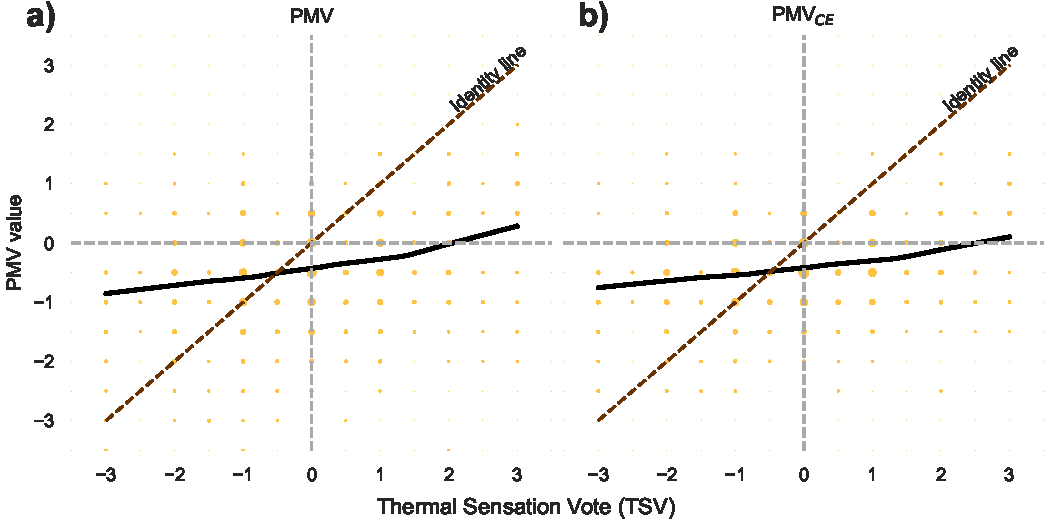
\includegraphics[width=\textwidth]{figures/bubble_models_vs_tsv_three_heights}
    \caption{Comparison between the \ac{pmv} and \ac{pmv-ce} models for the dataset with air speed measured at three heights. 
    The \ac{lowess} curve shows the relationship between the raw \ac{pmv} and \ac{tsv} data for the dataset with \ac{vr}~$\geq$~\qty{0.2}{\m\per\s} and measured at three heights.
    Raw data were then binned and a bubble chart (circle area is proportional to the number of votes in that bin) was superimposed over the regression curve to aid the visualization of a large dataset.
    The brown dashed line represents the identity line, where the slope is 1 and the intercept is 0.}
    \label{fig:bubble_models_vs_tsv_three_heights}
\end{figure*}
The \ac{pmv} model is more accurate than the \ac{pmv-ce} model.
The intercept of the \ac{pmv} model is \num{-.31} while the intercept of the \ac{pmv-ce} model is \num{-.41}.
Moreover, the \ac{pmv-ce} \ac{lowess} curve is only marginally higher than \num{0} despite participants reporting a \ac{tsv} of \num{3}.

The overall bias of the \ac{pmv} and \ac{pmv-ce} models is shown in Figure~\ref{fig:hist_discrepancies_three_heights}.
\begin{figure}[htb!]
    \centering
    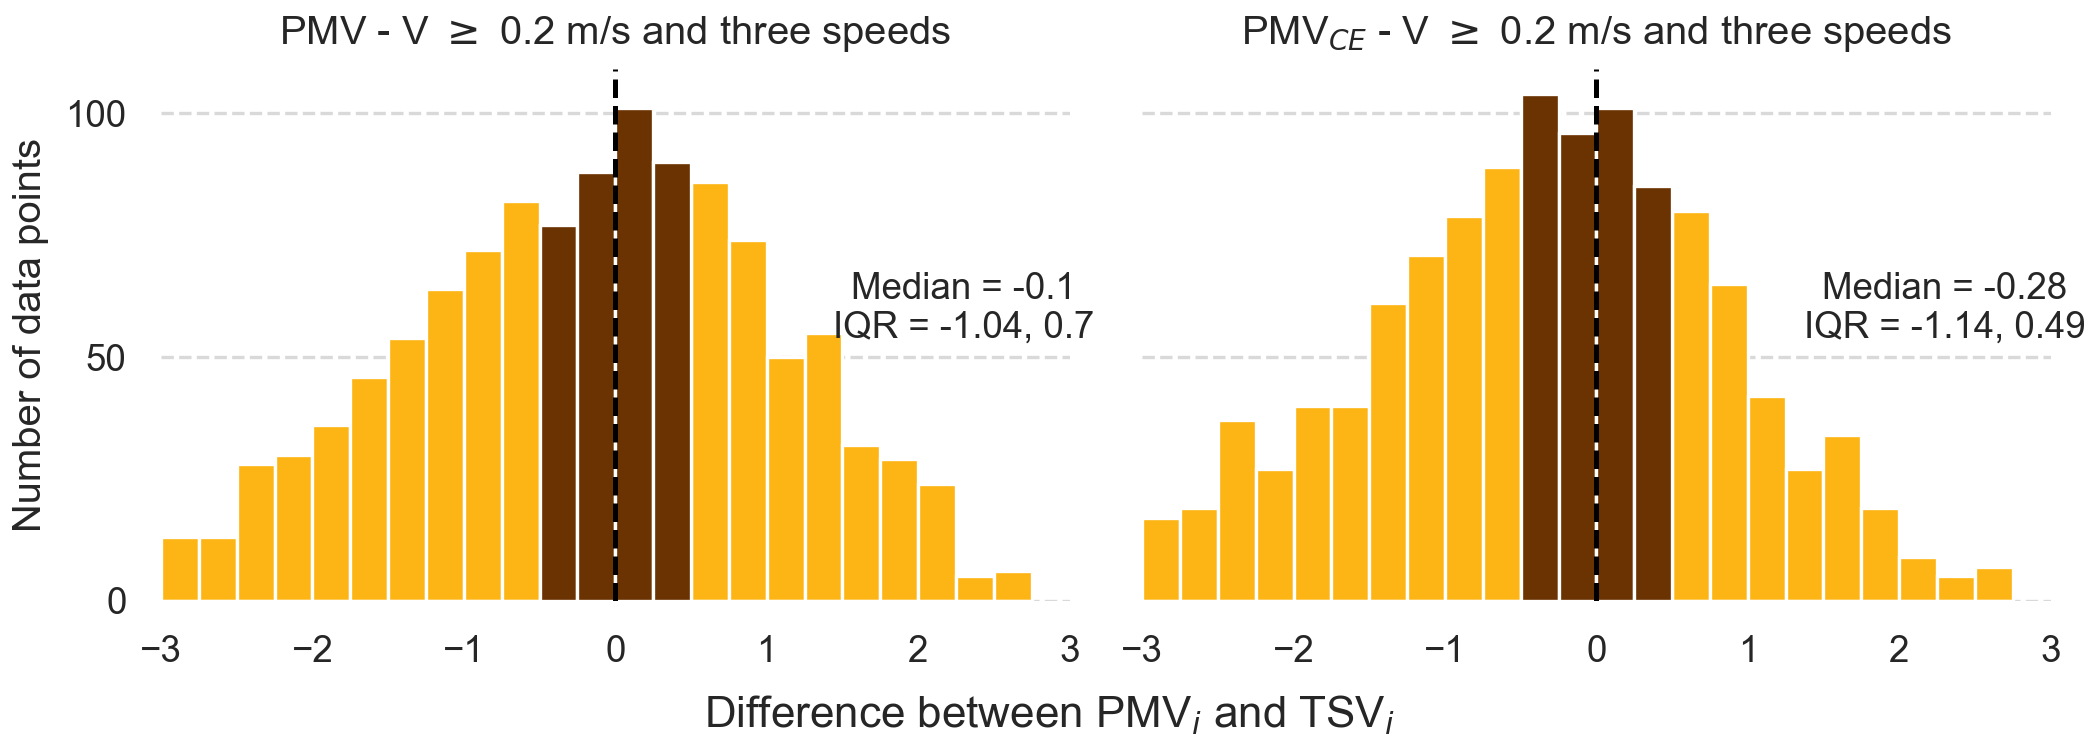
\includegraphics[width=\textwidth]{figures/hist_discrepancies_three_heights}
    \caption{Bias of the \ac{pmv} and \ac{pmv-ce} models for the dataset with air speed measured at three heights.}
    \label{fig:hist_discrepancies_three_heights}
\end{figure}
The \ac{pmv} model has a bias of \num{-.28} while the \ac{pmv-ce} model has a bias of \num{-.39}.
The interquartile range for the \ac{pmv} model is more centered around \num{0} than the \ac{pmv-ce} model.
These results allow us to conclude that the \ac{pmv} model is more accurate than the \ac{pmv-ce} model for the dataset with air speed measured at three heights.

\subsection{Dataset with \ac{vr} measured at three heights and \ac{tdb}~$\geq$~\qty{24}{\celsius}}\label{subsec:dataset-with-v-measured-at-three-heights-and-tdb-geq-24-celsius}
We are showing here the results for the subset of data with \ac{vr} measured at three heights and \ac{tdb}~$\geq$~\qty{24}{\celsius}.
We are reporting these results since the \ac{pmv-ce} aims to more accurately predict the thermal sensation, compared to the \ac{pmv}, when air movement is used to cool the occupants.
The results are shown in Figure~\ref{fig:hist_discrepancies_three_heights_limit_t}.
\begin{figure*}[htb!]
    \centering
    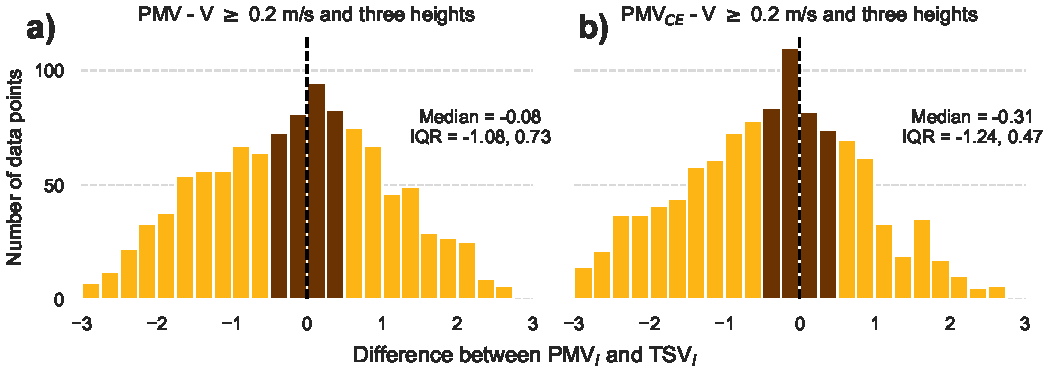
\includegraphics[width=\textwidth]{figures/hist_discrepancies_three_heights_limit_t}
    \caption{Bias of the \ac{pmv} and \ac{pmv-ce} models for the dataset with air speed measured at three heights and \ac{tdb}~$\geq$~\qty{24}{\celsius}.}
    \label{fig:hist_discrepancies_three_heights_limit_t}
\end{figure*}

The \ac{pmv} model has a bias of \num{-.08} while the \ac{pmv-ce} model has a bias of \num{-.31}. Even for this subset of data, the \ac{pmv} model is more accurate than the \ac{pmv-ce} model; this result is consistent with the previous analysis and confirms that the \ac{pmv} model is more accurate than the \ac{pmv-ce}.